% !TeX encoding = UTF-8
% !TeX program = xelatex

\documentclass[a5paper]{article} 
\usepackage{ctex}
\usepackage{indentfirst}
\usepackage{graphicx} 
\usepackage{subfigure}
\usepackage{verbatim}
\usepackage{geometry}
\usepackage{caption}
\usepackage{listings}
\usepackage{url}

\geometry{left=2.0cm,right=2.0cm,top=2.5cm,bottom=2.5cm}

\begin{document}

%基本信息%
\title{电教员的自我修养}
\author{YZ\_HL}
\date{2020.07.10}
\maketitle

%封面图标%
\begin{figure}[htbp]
\centering

\includegraphics[scale=0.3]{cover-p1.jpg}
\end{figure}

\thispagestyle{empty}
\newpage

%目录生成%
\tableofcontents
\thispagestyle{empty}
\newpage

\setcounter{page}{1}

%前言摘要%
\section{前言}
电教员,一个潜力无穷的职位,也是一个很忙,很考验人的职位。

ta或许会成为班内效率最高的工具人,ta或许会是美术设计的扛把子,ta或许会是班级交流的重要桥梁(天天去别的班修电脑)。
在高三生活中,我更感受到了一个优秀的电教员对于班内学习的推动能力是非常强大的,虽然这份努力常常是潜在不受人发觉的,但却是实实在在的。

个人认为,电教职业最考验的,是平衡的艺术——平衡自己的学业和职业,平衡不同同学间的不同需求,在最短的时间内实现最大的增效。怎么做到抓大放小,精准突破,仍需实际的磨砺才能深刻体会。

毛泽东先生曾言:“我们的文学艺术都是为人民大众的”,电脑技术也是如此。
在电教生活中应时刻铭记自己是为落实多数人的需求而工作的,而不是为了自娱自乐。

编写这一手册,不仅仅是为了指出实用的软件是什么,而更是渗透我认为在完成这项工作的过程中,
所应具备的核心素养——发现问题,寻求方案,解决问题的能力。

下面将以几个我就职期间的典型例子来讲述如何更好的做好电教工作,
注意,我所讲述的典例并不会只是单纯聚焦在这点中,
而是会发散出一些可以改进的发展方向,以及渗透我的一些思考方式在内。

强烈建议配合百度慢慢去实现,选择了电教员这个职业,不应只是满足于最基本的要求,而更要有着敬业的精神。

另外再强调一点,我们不能追求纯粹的技术主义,纯粹的技术主义是非常可怕的,最典型的案例便是"万湖会议",希望阅读这本小册子的你,
能够在人文主义的关怀下,热爱人,敬爱人,用技术去造福人。

希望阅读愉快,能够对你有用。

【本手册所叙述的内容以2020.07.10时为准,此时教室电脑未更换带还原卡的电子白板,未更新讲台设施】
\newpage

%正文部分%
%第一小节%
\section{典例回顾}
    \subsection{Everything/Listary 效率的提升是成功的开始}
        关于这两款软件大家应早有耳闻,同为一定程度上取代Windows自带缓慢搜索的软件哪一款更加适合校园生活?

        个人认为Everything更合适。下面列举出三年我实操的感受,希望能帮助你们做决定。
        \subsubsection{使用背景}
            学校的课件库是基于Windows文件共享所搭建的网络共享文件夹,一个老师持有一个账号,而学生使用通用的只有读取权限的账号进行访问。
            这种机制使得学生容易在重重子文件夹中迷失方向难以达到目的,较多优秀资料积累在课件库待挖掘(初期会有点累,成熟后效果还是很不错的)。

            观察可知同学们搜索的痛点主要出现在两个场景,一为课间多同学希望再看一下上课的课件,二为下午练/周测后难以寻找到答案电子版,究其根本都是难以在短时间内找到所需要的文件。

            为了解决这个问题,我们锁定了这两款工具,然后第一步是比对搜索速度和搜索方式,第二步是比对易用程度和使用门槛,以确定最终选择。
        \subsubsection{搜索速度和搜索方式}
            在搜索速度上,两款软件难争上下,都能够提供几乎“秒搜”的响应,但是代价都是一定程度的延迟(可通过满缓存检测和定期检测解决)。

            在搜索方式上,Everything是双击打开直接搜索或者右键从当前目录开始搜索,而Listary可以做到双击Ctrl键自动唤醒进行搜索,在方便性上Listary胜一筹。

            在搜索匹配中,Everything对于通配符和正则表达式的支持比Listary要好很多,这对于筛选某类文件(例如'*.mp4 | *.flv'便可以很容易搜索出两大类视频文件)有着重要意义。

            诚然,Listary还有许多很棒的功能(例如'bd 蒟蒻'即是用百度搜索搜索‘蒟蒻’这个关键词),但是在没有网络的教室电脑上这些拓展功能不如专注于做搜索的Everything。
        
            另外,Everything具有搭建http服务器和ETP服务器(可以连接别人的Everything索引)的能力,你可以在设置账号密码后,在校内任何一部机器通过浏览器或Everything访问班内索引的文件夹,这对于电教员来说也比较有用。
        \subsubsection{易用程度和使用门槛}
            要知道,绝大多数同学都难以像你一样能够较为娴熟的运用这些工具提高生产力。因此选用门槛较低更为易用的方案是非常重要的。

            除去搜索时关键词的运用,我们来比对一下搜索时两款软件的使用体验:

            Listary的可定制性更高,功能并不局限于搜索,双击Ctrl搜索对普通同学很友好。但是,非常容易误触发,课上弹出搜索框的感觉总容易让人窒息。

            Everything主攻搜索,集成在右键菜单的搜索相较来说麻烦一些,但是,以我经验看使用门槛不算太高(两年使用时间班内同学基本都能独立完成搜索)。

            杀鸡焉用牛刀,在我看来,使用Everything已经足够应付校内局域网环境的文件搜索需求。
        \subsubsection{Everything的基础配置}
            初始化时,我们建议你选用“安装Everything服务”,而非以管理员身份运行。这是为了适应在日常使用中,维护系统安全和便于管理而使用非管理员账号的举措。
            若初始化时设置错误,可在菜单栏"设置"->"选项"->"常规"中,找到对应选项并勾选/去勾选(建议启动开机自启,避免在想要搜索时才进行预扫描耽误时间)。
            
            然后,建议打开筛选器,平时查询课件时可将筛选器设置为"文档",需要搜索阅读课视频(力推《这就是中国》)时同理设置,便于过滤无效信息,查询锁定。

            两个设置位置如下图所示:

            \begin{figure}[htbp]
            \centering
            \begin{minipage}[t]{0.44\textwidth}
            \centering
            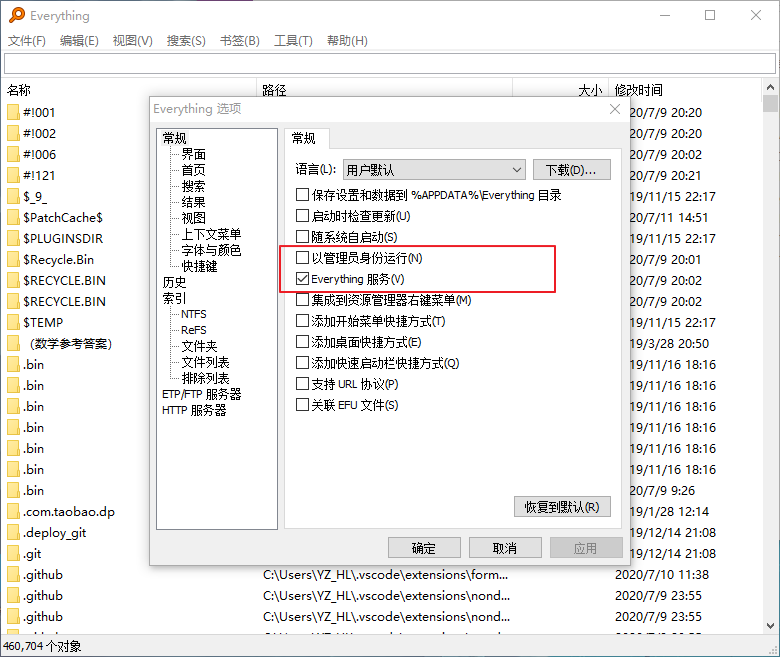
\includegraphics[scale=0.20]{2.1-p1.png}
            \end{minipage}
            \begin{minipage}[t]{0.44\textwidth}
            \centering
            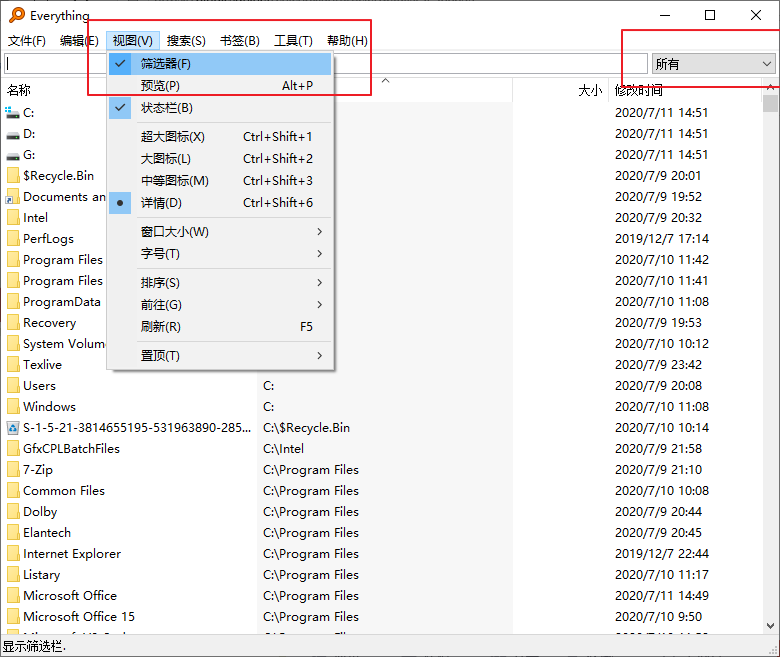
\includegraphics[scale=0.20]{2.1-p2.png}
            \end{minipage}
            \end{figure}

            现在,最重要的一步是添加课件库到索引中,
            这一步可以通过先映射网络驱动器后添加驱动器号到索引中实现,也可以直接输入对应的网络路径实现。
            
            但记住这需要保存你登陆到课件库的账号和密码,不然即使设置了"开机自启/定时搜索"都不能够实现。
            
            以理科教学资源库的连接为例,如后文图中所示。

            文科教学资源库,政体处同理设置即可。

            添加索引后按照指示和班级需求配置“尝试监控变化”,注意时间间隔不要设置太短,对系统的资源消耗会比较大。

            \begin{figure}[htbp]
            \centering
            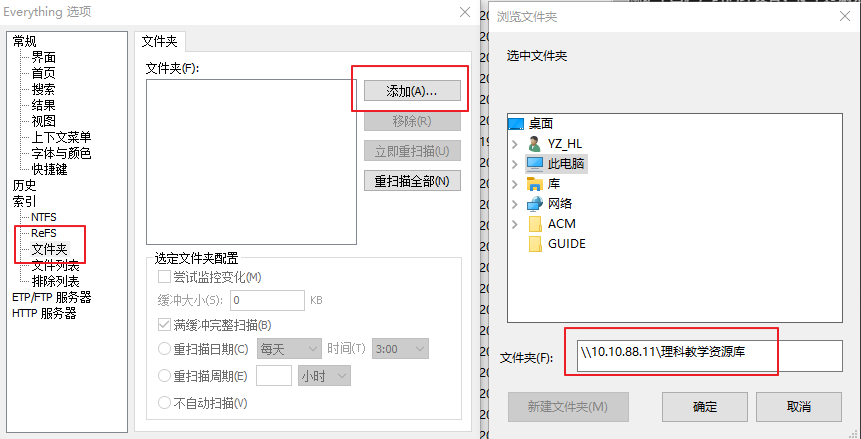
\includegraphics[scale=0.3]{2.1-p3.png}
            \end{figure}

            你可以使用ProcessLasso来辅助你调控任务优先级和资源占用率,防止由于Everything占用过多影响了正常上课。

            到此,最基本的Everything配置已经完成,其他设置可以自行摸索。
            
        \subsubsection{Everything及衍生的拓展应用}
        举个例子,你可以在班内组建一套无线网络,电脑首先连接该网络,
        在开启Everything的Http服务器后,同连接该网络的各种电子设备(手机,平板等)均可通过以"http://ip地址"的形式来访问该服务,
        这将有利于周末期间缓解多人同时使用电脑查看课件的压力(连接wifi后可以使用自己的设备来访问)。
        
        若不采用Everything方案,连接wifi后的电子设备也可以通过安装"ES文件浏览器"来直接访问课件库,
        但是主要操作者会变为普通学生,使过程变得更加繁琐,容易出错。
        
        不过对于教室的电视(基于安卓系统定制)来说,可以利用adb远程连接安装该应用并设置为开机自启,实现电视访问课件库,
        这有利于午休期间利用遥控器(若无遥控器可使用adb操控)访问课件抄笔记减小电脑使用压力,
        且在晚修投放教师指定的题目(一般需要开投影)时不影响正常的电脑使用。

        以上想法我均已实现并得到良好反响。

        很多时候,一个你想要实现的想法往往能变成一套需要实现的系统,但是不论如何,都必须要切实符合同学们的利益,而非自娱自乐。
    \newpage

    \subsection{OfficeToPDF "轮子"的进一步开发与模型化}
        OfficeToPDF,即是将doc/docx/ppt/pptx等文档格式转为PDF,一般单个文件的转换可以使用Office直接导出(WPS Office部分版本需要付费,建议使用党政机关版本,Logo可改,功能齐全)
        或者配合虚拟打印机(Microsoft Print PDF)来实现,Office本身不支持批量转换,网络上批量转换文件的工具普遍有失败率高,版本较旧,高额付费,难以适应等问题。

        \subsubsection{使用背景 \& 后续效果}
        在校内,导出的PDF文件一般配合"合法"的Kindle,ireader阅读器来使用,一般用途为抄笔记,排队时背单词,偶尔看看小说(此处堵不如疏)。

        高二上学期,班内阅读器只有两三部,成为了非常抢手的学习工具,曾有一段时间我个人的ireader自己都不知道借给了谁。

        那时,使用者的主要矛盾集中在难以搜索到想要的文件(上一小节已解决)和同学们利用office的导出一个个手动转换非常耗时。
        我意识到,如果提供良好强大的软件辅助批量转换,在初心为借助该工具用于学习的有意向人群中,班内阅读器数目会大幅上涨,
        一方面带来更高的学习效率,另一方面会带来许多的小说加剧同学们的颓废。那时我决心在利用信息技术对小说的严格管控下提供良好的软件生态。

        后面发展的确如所料,高二下学期,我班阅读器达到十五部,其中虽然仍有两部常用于沉迷小说(莫得管,从mp3过渡到Kindle罢了),
        但切实帮助了余下十三位同学以更高效率来学习,以及让原本持有阅读器的两三位同学能够安稳使用阅读器,而不需要天天被借走。
        
        阅读器数量不用太多,不需要做到人手一部,一般一个人很少高频率一直去使用它的设备,十五到二十部已经足够班内大部分同学使用。

        阅读器效率最高的时候大概是高三,彼时我已建立起"精选资料库"和"答案库",同学们不需要离开座位走上讲台进行搜索
        (搜索软件入门使用很简单,此时搜索的关键词成为大部分同学的效率瓶颈),
        打开自己或同桌的阅读器,就可以查阅想要的资料,免去了搜索的烦恼,同时,早午读有阅读器的同学快速开始阅读不需费时间找卷子,
        总体来说这是利大于弊的,有利于同学们更快更准的学习,不必为过多琐事分心。

        补充一下,我在最初建立这套软件生态时,没有料到后面可以发掘出
        生词本电子化(输入生词/提取生词并重排为带有原词,释义,音标,音频的单词表的电子文件),
        定期自动推送化(扫描指定路径更新的文件并自动转为PDF,通过邮箱推送(Kindle)或通过网页传输(ireader)来实现自动化推送最新课件)
        的使用方法。

        \begin{figure}[htbp]
        \centering
        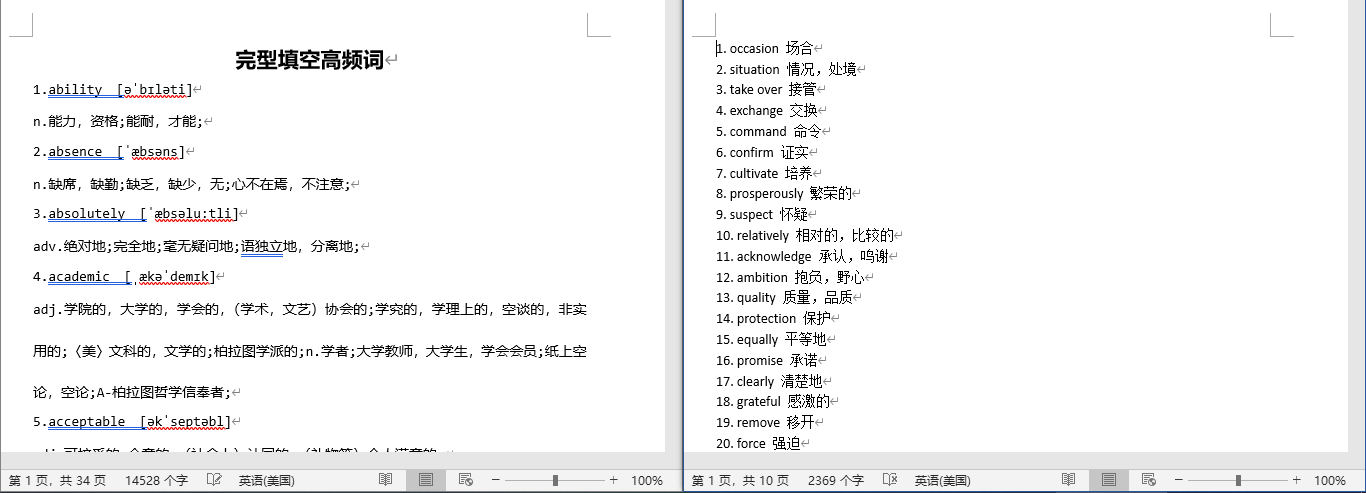
\includegraphics[scale=0.2]{2.2-p1.png}
        \caption*{单词表前后生成对比}
        \end{figure}

        这告诉我们,有的时候要放胆去做,相信1+1>2,
        我们难以想象未来,就像4G标准刚出时我们难以想象这会带来多大的流量浪潮。
        现在你所完成的每一套生态,所含的意义不会是单单实现一个目的,在
        未来的某个瞬间,你或许会在写类似"轮子"的时候能够直接套用加快开发,也或许会在某天灵感迸发时在原有基础上添砖加瓦实现如虎添翼的效果。
        但这一切的基础,都是你去做了,并且切中要害了。

        PS:邮箱定期推送建议使用SMTP去实现,可能会好实现一些,无线网络直推需要结合抓包软件分析数据包格式并定向发送。

        \subsubsection{寻找方法 \& 初步完成}
        使用环境:Windows10教育版,WPS 2019专业版;

        通过百度,我比对了大多数网上能看到的office批量转换软件,
        发现大部分使用的都是多次调用Office接口的方法来实现批量转换。
        此时,选择利用Microsoft的vbs脚本进行核心调用是不错的选择。
        
        在搜寻相关写过该种方法的博客和微软官方给出的VBS函数接口文档后,修改完善核心代码如下:

        \begin{figure}[htbp]
        \centering
        \begin{minipage}[t]{0.49\textwidth}
        \centering
        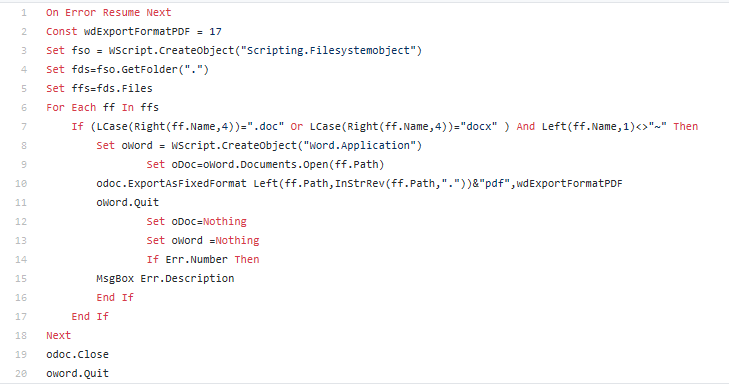
\includegraphics[scale=0.2]{2.2-p2.png}
        \caption*{word\_to\_pdf.vbs}
        \end{minipage}
        \begin{minipage}[t]{0.49\textwidth}
        \centering
        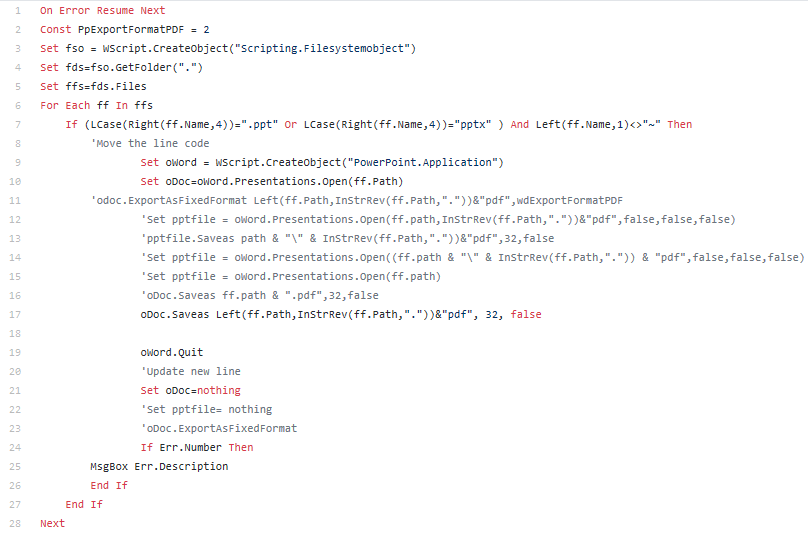
\includegraphics[scale=0.2]{2.2-p3.png}
        \caption*{ppt\_to\_pdf.vbs}
        \end{minipage}
        \end{figure}

        两份代码均在\url{https://github.com/YZ-HL/OtherCodes/tree/master/Office%20To%20PDF}中能找到并下载。

        注:该两份代码是直接修改而来,语法风格和效率上或许会有些小问题。但在有限时间内,能用就好。

        而后,初步实现的效果是:

        \begin{figure}[htbp]
        \centering
        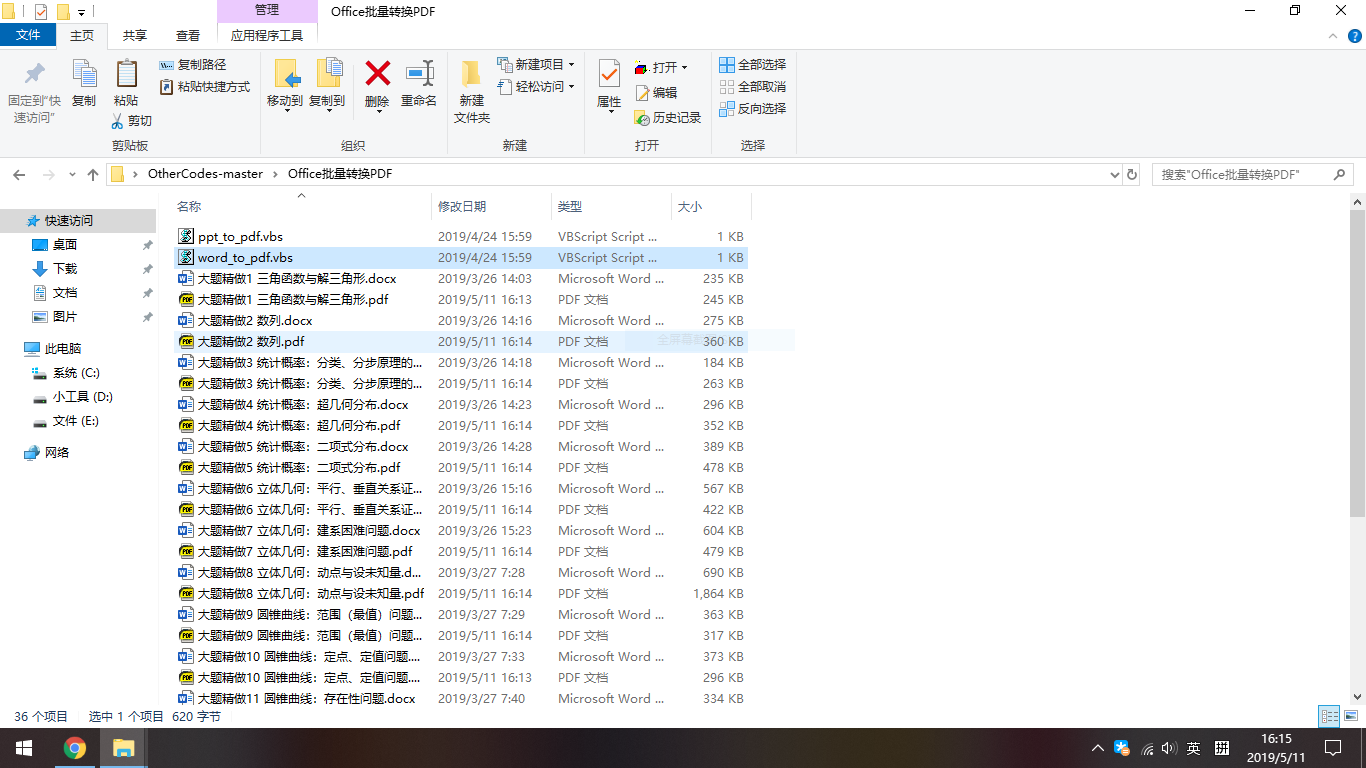
\includegraphics[scale=0.3]{2.2-p4.png}
        \end{figure}

        到这,我们已经初步实现了批量转换功能。问题是,怎么才能降低使用门槛,使得它变得更易用,更好用?

        \subsubsection{降低使用门槛 \& 空间自动回收}
        分析使用时可能会遇到的问题,大概分成两类,一为误移动删除vbs文件,二为转换完拷走PDF后若不删除将会重复转换,极大降低效率。
        此时,利用Python和bat脚本外套一层用户指引层成为了一个比较好的选择。进一步这也便于记录日志文件,以检测重复转换,可视化批量转换使用率等等。

        PS:Python其实也有office转换的调用库封装,但是win32库之前调炸了所以这里就只利用Python和bat来进行用户操作和文件操作。

        为了给用户一个显眼的标识,我们创建一个主程序的快捷方式,并且更改图标,使其变得突出。

        接下来分析主程序,由于时间有限,我们只要实现一个简单的引导就好了,大概思路如下:

        1.程序展示操作指引后进入暂停状态,然后"按任意键继续程序";
        
        2.继续程序后继续转换,转换完毕后归类到以当日日期为名称的文件夹内(以日期为分类便于空间回收);
        
        3.归类完毕后检测是否有名称对应N日前日期的文件夹,若存在,则删除,一方面回收空间,另一方面防止文件夹过多影响用户体验;

        4.写入日志文件,记录何时转换了什么文件,便于评估该程序是否符合需求,还有没有进一步开发的必要。且这部分数据可以用于拓展程序功能。

        归结四大步后,完善程序便也不难了。建议使用Python进行编写,实现功能简单易上手。

        源程序由于我放在学校忘记拷出来了所以没有了...
        
        \subsubsection{将系统模型化}
        我们在上面的程序中,已经实现了对于批量转换的分类归档空间回收。

        那么,我们是否可以把这个程序所基于的模型迁移到其他地方去呢?答案是肯定的。

        对于Kindle用户,epub格式不受支持让其难以拷贝一些电子书,你可以采用类似Caliber的强大一站式软件进行转换,
        也可以利用官方的KindleGen(原本只支持单文件转换),套上上面的模型,实现批量转换。

        思路如下:

        1.扫描整个目录下需要转换的文件的文件名并记录

        2.查看KindleGen的调用格式,明白其文件名变量该如何填入调用命令中
        
        3.利用程序逐条执行调用命令,例如:
        
        \begin{lstlisting}[language={python}]
            for i in 文件名列表:
                nf = i+".mobi"
                os.system("KindleGen.exe i -o "+nf)
        \end{lstlisting}

        这便完成了一次简单的迁移。

        同理,我们也可以用于简单的桌面的杂项文件清理。
        
        只需要定义排除列表排除科任老师的快捷方式及某段时间内新增必须放桌面的文件,
        然后每日开机时利用Windows自带的任务计划程序,
        将其他临时存放在桌面的文件归类到某文件夹内,
        保留三天后删除,就可以保证每天桌面的整洁。

        这三种开发要求看似毫无联系,实则殊途同归。

        这便是模型化意识,在这样意识的指导下,1+1>2。

    \section{杂七杂八——别的一些小改进}
        \subsection{小型课件库 | 文件共享服务器的搭建}
        一般,教室电脑均采用Windows系统,此时,实现文件共享只需要简单几步。
        
        1.获取管理员权限,创建专用的访问共享文件夹的账号,设置为不允许登录(安全策略)及隐藏(注册表)。
        
        !设置为密码永不过期,不然容易出现用了一半就要求修改密码的情况,坏兴致
        
        2.右键想要共享的文件夹,点入文件夹属性,在高级共享中确定你想要共享的对象和权限设置。
        
        !注意,安全选项卡内的权限设置要与你共享对象权限设置一致,不然容易出现拒绝访问的情况

        3.本机检查\url{\\127.0.0.1},看共享文件夹是否已经出现,再去别班电脑尝试访问一下。
        
        !如果需要测试权限可以右键映射网络驱动器,选用其他账号登陆,输入你预先设定的账户即可

        对此的应用比较广:
        
        你可以在接入内网的任何一部电脑上访问你班内的文件,跑一些绿色版程序;

        你可以联系教师提供专供通道直达你班,放一些可能涉及班内信息不想透露的文件(比如各种有密码的PPT里面往往就是各种照片和回忆),
        不走主课件库老师可以不用再设置密码,以防忘记(是的,我前英语老师各种PPT的密码我记得比她还清楚呜呜呜);
        
        你可以让老师放一些课件库放不下的视频(课件库每个老师的账号的存储空间有一定限额,如果你自己开共享文件共享100G都轻松啦~);

        你可以和几个小伙伴一起,组建民间资料库并维护(某竞赛前民间资料库主要由我维护,能够灵活及时更新各种最新信息,提供了很大帮助);

        ...

        能够怎么做,取决于你想要去怎么做,但是注意,抓大放小,莫陷入其中误了大事。

        \subsection{考勤自动填充 | 避免重复工作非常有用}

        作为一班之电教员,很可能也要承担起考勤的任务。这需要你每日在9:00前上报本班缺勤情况及其原因。

        工作不是什么新奇工作,但是在输入缺勤信息时,总要输入缺勤人的固定的个人信息(电话号码,宿舍号,性别等),有没有什么办法自动化?

        当然有。在这个问题中,我预先将个人信息以一定格式存在csv文件中,
        后采用了输入学号的方式锁定个人信息,并利用Python的库进行自动填充;

        后来,由于电脑性能较差(2G小内存),开浏览器都卡,于是进行流量分析直接用Python发送Post请求完成考勤;

        !可以借助Fiddler等工具辅助分析保存结果,既然是上传文件就注意Post中较大流量的部分就好了,确定上传方式即可。

        再后来,完善自动考勤系统,在无人登记缺勤时程序自动定时上传考勤结果,实现双手几乎完全解放。

        这有着一个循序渐进的过程,若没有开始的设想,便没有最后的解放,因此,敢想,敢做,是非常重要的。

        开始写考勤程序之前我还完全没有接触过Python语言,恰逢周六,我学了两天,口胡了一个雏形出来。后面程序带回学校,
        又过了两天,前前后后测试考勤了二十来次,就基本能用了。所以不需要说畏难,曾经我也是0基础,想去做,认真去做,
        写出一个功能还是很简单的事情。

        部分效果 \& 上送部分源码:

        \begin{figure}[htbp]
        \centering
        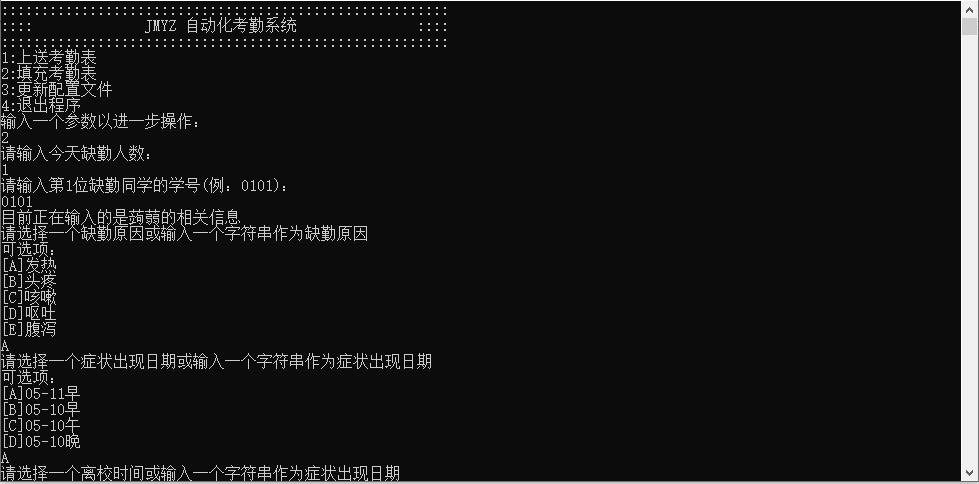
\includegraphics[scale=0.30]{2.3-p3.png}
        \end{figure}

        \begin{figure}[htbp]
        \centering
        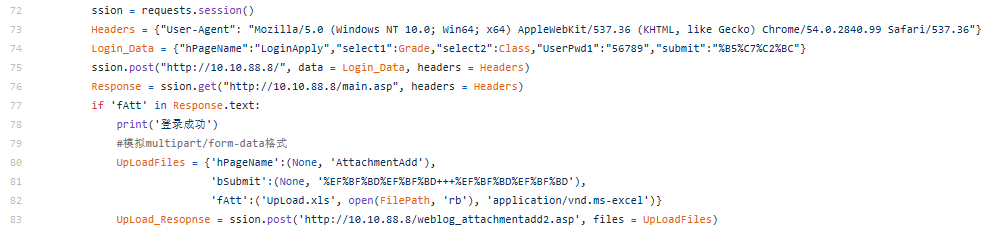
\includegraphics[scale=0.30]{2.3-p2.png}
        \end{figure}

        \subsection{软件推荐清单}
        此处不再做详细解释了,只是列举一些可能较好用的软件:

        【Mamsds桌面倒计时】样式丰富,美观大方,高考必备;

        【雨滴】桌面美化用,有丰富的拓展,可用于课程表的展示;

        【Potplayer】强大的播放器,支持解码格式多;

        【Dism++】系统优化,系统备份必备,重装系统也可以通过该软件进入RE模式进行;

        【微PE】纯净系统PE,不捆绑,建议对于校内电脑使用"全能单分区"模型进行U盘烧录,兼容性较好;

        【Renamer】高级的批量重命名软件,有绿色版,能够很方便裁掉一些不需要的部分,PDF拷到Kindle内不怕因为文件名太长而看不见关键信息;

        实例展示见下页。

        \begin{figure}[htbp]
        \centering
        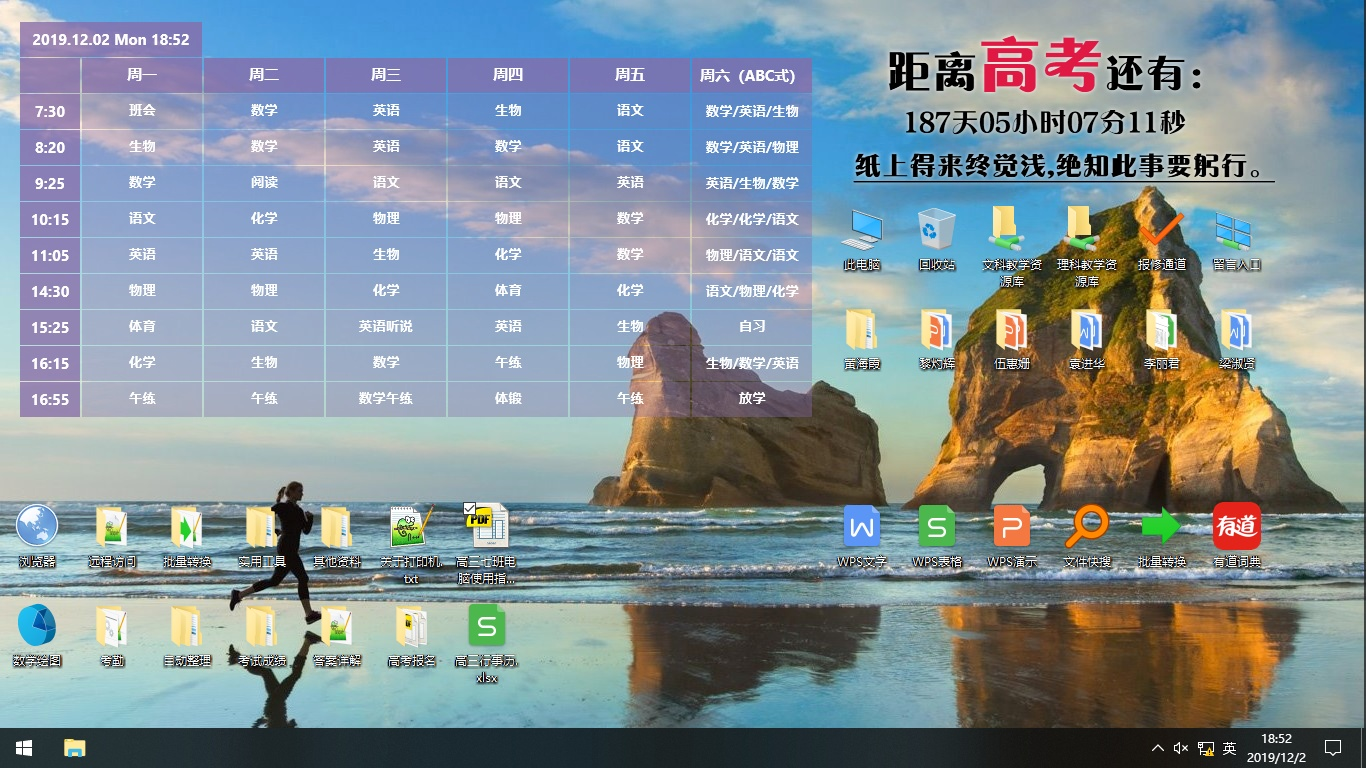
\includegraphics[scale=0.25]{2.3-p4.png}
        \caption{课程表与倒计时}
        \end{figure}

        \begin{figure}[htbp]
        \centering
        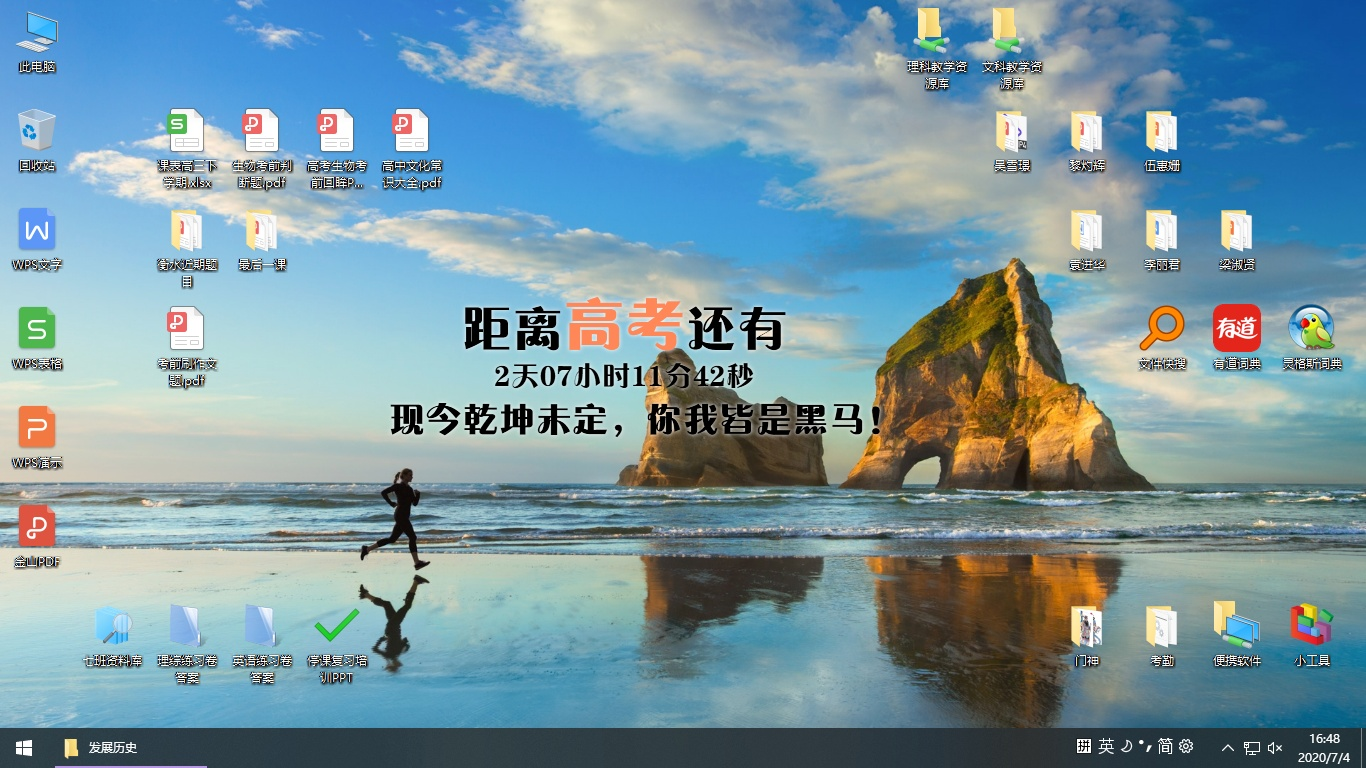
\includegraphics[scale=0.25]{2.3-p5.png}
        \caption{最后两天}
        \end{figure}

        PS:倒计时使用字体为"方正粗活意简体",由红色转为黄色代表接下来的高考将会一路绿灯( •̀ ω •́ )✧。

    \newpage

    \section{后记}
        吾辈电教,当有"敢教日月换新天"的勇气,当有"长风破浪会有时"的信心,当有"功成不必在我,功成必定有我"的觉悟,
        希望你们能够在这条路上走出属于自己的光华璀璨!

        送一段我以前比较喜欢的歌词:\\ \\

        如果标算太难请坚定信念,

        不如回头再看一眼题面,
        
        以那暴力模拟向正解吊唁,
        
        蒟蒻的蜕变,
        
        神犇出现,
        
        终将与梦想擦肩。

        ——《膜你抄》选段,有删改 \\ \\

        本文档发布于:\url{https://github.com/YZ-HL/Guide/tree/master},欢迎过去点小星星~~

        最后希望多一些小姐姐也能参与其中(本来高二还有两个的,高三全年级就只剩我了,小声bb)

        互助交流的话请先联系我邮箱\url{yz_hl@oi-liu.com},不直接放微信/QQ是希望稍微筛选一下啦...

        (¬‿¬)

        Powered By \LaTeX

\end{document}